% Generated by pysimcount.figleader -- do not edit; regenerate instead.
% figure: main-cnot-all-formulas -- cost at n = 500, one row per formula
% seeds [1, 2, 3, 4, 5, 6, 7, 8, 9, 10]; metric=cnot kind=xyz merged (Clifford+Rz (cz), simcount template)
% shown: suzuki4, suzuki6, mo-q6, mo-q14, bm-q10, mo-o8-q21, morales-y8m10, morales-m8
% removed (see main-cnot-all-formulas-ranking.md): lie-trotter, suzuki2, suzuki8
% n = 500; x = the source record's plotted value; bars min..max over seeds
% cheapest on = seeds on which the formula is cheapest; rank range = min..max of its rank over seeds
% per-seed values: runs' totals if measured, else each seed's own fit c(n) ceil(a_s n^b_s)
% row order (plotted value) ['bm-q10', 'morales-m8', 'mo-q14', 'morales-y8m10', 'mo-q6', 'mo-o8-q21', 'suzuki6', 'suzuki4'] differs from mean-rank order ['morales-m8', 'bm-q10', 'mo-q14', 'morales-y8m10', 'mo-q6', 'mo-o8-q21', 'suzuki6', 'suzuki4']
% derived: main-cnot-all-formulas.json by pysimcount.figleader; source_sha256=89709f32a81a149627fa77a011518b188e319f292a4b8a71e0fe77cca50974a7
% figure made at git_commit=eed0c490bd2a7ed3c821acf76ae930c79d2195f6 git_dirty=False
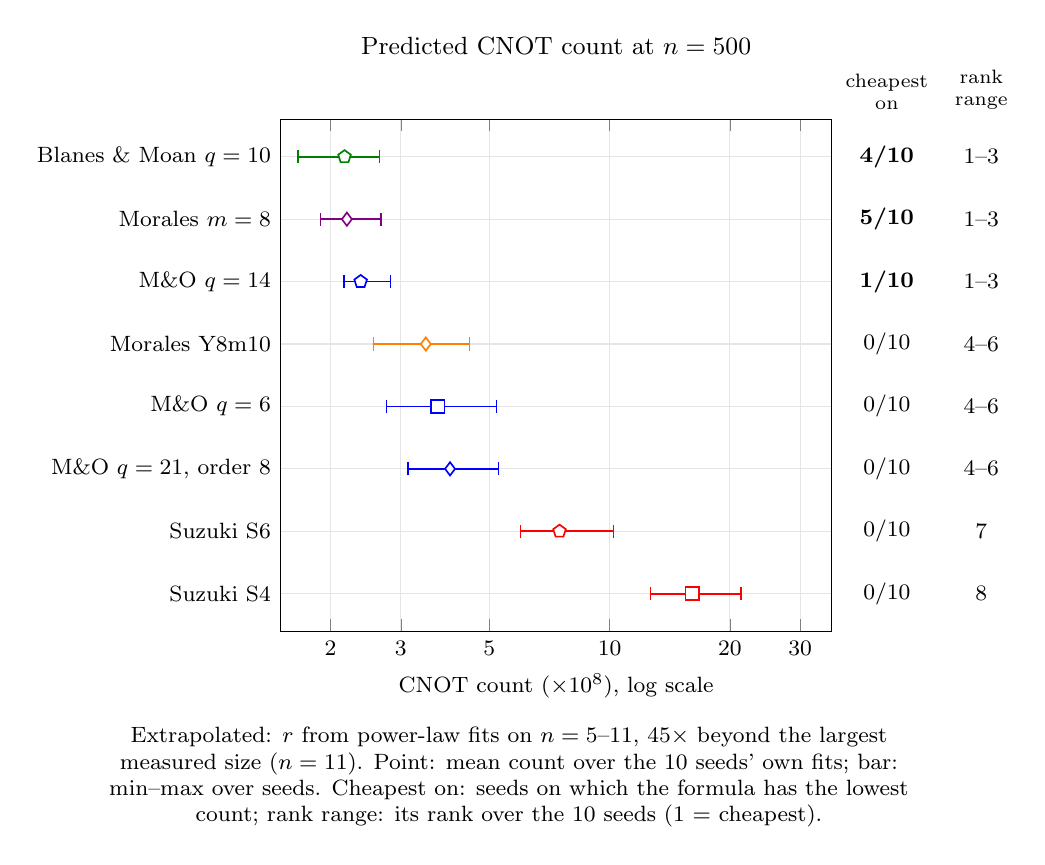
\begin{tikzpicture}
  \begin{semilogxaxis}[
    scale only axis, clip=false,
    at={(0cm,0cm)}, anchor=south west,
    width=7.0cm, height=6.5cm,
    title={Predicted CNOT count at $n = 500$}, title style={font=\small, yshift=14pt},
    xlabel={CNOT count ($\times 10^{8}$), log scale}, xlabel style={font=\footnotesize},
    xmin=1.5e+08, xmax=3.6e+09, xtick={2e+08,3e+08,5e+08,1e+09,2e+09,3e+09}, xticklabels={2,3,5,10,20,30},
    xminorticks=false,
    y dir=reverse, ymin=0.4, ymax=8.6, ytick={1,2,3,4,5,6,7,8},
    yticklabels={{Blanes \& Moan $q=10$},{Morales $m=8$},{M\&O $q=14$},{Morales Y8m10},{M\&O $q=6$},{M\&O $q=21$, order 8},{Suzuki S6},{Suzuki S4}},
    tick label style={font=\footnotesize}, ytick style={draw=none},
    xmajorgrids=true, ymajorgrids=true, grid style={black!10},
  ]
    % bm-q10: plotted 2.16874e+08, seeds 1.65886e+08..2.65106e+08, cheapest on 4/10, rank 1..3
    \addplot[green!50!black, only marks, mark=pentagon*, mark size=2.4pt, mark options={solid, fill=white, line width=0.6pt}, error bars/.cd, x dir=both, x explicit, error bar style={solid, line width=0.6pt}] coordinates {
      (2.16874e+08,1) += (4.82324e+07,0) -= (5.09876e+07,0)
    };
    % morales-m8: plotted 2.19834e+08, seeds 1.89336e+08..2.67651e+08, cheapest on 5/10, rank 1..3
    \addplot[violet, only marks, mark=diamond*, mark size=2.4pt, mark options={solid, fill=white, line width=0.6pt}, error bars/.cd, x dir=both, x explicit, error bar style={solid, line width=0.6pt}] coordinates {
      (2.19834e+08,2) += (4.7817e+07,0) -= (3.0498e+07,0)
    };
    % mo-q14: plotted 2.37981e+08, seeds 2.16201e+08..2.82036e+08, cheapest on 1/10, rank 1..3
    \addplot[blue, only marks, mark=pentagon*, mark size=2.4pt, mark options={solid, fill=white, line width=0.6pt}, error bars/.cd, x dir=both, x explicit, error bar style={solid, line width=0.6pt}] coordinates {
      (2.37981e+08,3) += (4.40553e+07,0) -= (2.17797e+07,0)
    };
    % morales-y8m10: plotted 3.46477e+08, seeds 2.56615e+08..4.4489e+08, cheapest on 0/10, rank 4..6
    \addplot[orange, only marks, mark=diamond*, mark size=2.4pt, mark options={solid, fill=white, line width=0.6pt}, error bars/.cd, x dir=both, x explicit, error bar style={solid, line width=0.6pt}] coordinates {
      (3.46477e+08,4) += (9.8413e+07,0) -= (8.9862e+07,0)
    };
    % mo-q6: plotted 3.71342e+08, seeds 2.758e+08..5.21575e+08, cheapest on 0/10, rank 4..6
    \addplot[blue, only marks, mark=square*, mark size=2.4pt, mark options={solid, fill=white, line width=0.6pt}, error bars/.cd, x dir=both, x explicit, error bar style={solid, line width=0.6pt}] coordinates {
      (3.71342e+08,5) += (1.50232e+08,0) -= (9.55425e+07,0)
    };
    % mo-o8-q21: plotted 3.98548e+08, seeds 3.12715e+08..5.27085e+08, cheapest on 0/10, rank 4..6
    \addplot[blue, only marks, mark=diamond*, mark size=2.4pt, mark options={solid, fill=white, line width=0.6pt}, error bars/.cd, x dir=both, x explicit, error bar style={solid, line width=0.6pt}] coordinates {
      (3.98548e+08,6) += (1.28537e+08,0) -= (8.5833e+07,0)
    };
    % suzuki6: plotted 7.49087e+08, seeds 5.98829e+08..1.02475e+09, cheapest on 0/10, rank 7..7
    \addplot[red, only marks, mark=pentagon*, mark size=2.4pt, mark options={solid, fill=white, line width=0.6pt}, error bars/.cd, x dir=both, x explicit, error bar style={solid, line width=0.6pt}] coordinates {
      (7.49087e+08,7) += (2.75659e+08,0) -= (1.50258e+08,0)
    };
    % suzuki4: plotted 1.60899e+09, seeds 1.26284e+09..2.13375e+09, cheapest on 0/10, rank 8..8
    \addplot[red, only marks, mark=square*, mark size=2.4pt, mark options={solid, fill=white, line width=0.6pt}, error bars/.cd, x dir=both, x explicit, error bar style={solid, line width=0.6pt}] coordinates {
      (1.60899e+09,8) += (5.24758e+08,0) -= (3.46154e+08,0)
    };
    \node[anchor=south, font=\scriptsize, align=center] at ([xshift=0.7cm]axis cs:3.6e+09,0.4) {cheapest\\on};
    \node[anchor=south, font=\scriptsize, align=center] at ([xshift=1.9cm]axis cs:3.6e+09,0.4) {rank\\range};
    \node[font=\footnotesize\bfseries] at ([xshift=0.7cm]axis cs:3.6e+09,1) {4/10};
    \node[font=\footnotesize] at ([xshift=1.9cm]axis cs:3.6e+09,1) {1--3};
    \node[font=\footnotesize\bfseries] at ([xshift=0.7cm]axis cs:3.6e+09,2) {5/10};
    \node[font=\footnotesize] at ([xshift=1.9cm]axis cs:3.6e+09,2) {1--3};
    \node[font=\footnotesize\bfseries] at ([xshift=0.7cm]axis cs:3.6e+09,3) {1/10};
    \node[font=\footnotesize] at ([xshift=1.9cm]axis cs:3.6e+09,3) {1--3};
    \node[font=\footnotesize] at ([xshift=0.7cm]axis cs:3.6e+09,4) {0/10};
    \node[font=\footnotesize] at ([xshift=1.9cm]axis cs:3.6e+09,4) {4--6};
    \node[font=\footnotesize] at ([xshift=0.7cm]axis cs:3.6e+09,5) {0/10};
    \node[font=\footnotesize] at ([xshift=1.9cm]axis cs:3.6e+09,5) {4--6};
    \node[font=\footnotesize] at ([xshift=0.7cm]axis cs:3.6e+09,6) {0/10};
    \node[font=\footnotesize] at ([xshift=1.9cm]axis cs:3.6e+09,6) {4--6};
    \node[font=\footnotesize] at ([xshift=0.7cm]axis cs:3.6e+09,7) {0/10};
    \node[font=\footnotesize] at ([xshift=1.9cm]axis cs:3.6e+09,7) {7};
    \node[font=\footnotesize] at ([xshift=0.7cm]axis cs:3.6e+09,8) {0/10};
    \node[font=\footnotesize] at ([xshift=1.9cm]axis cs:3.6e+09,8) {8};
  \end{semilogxaxis}
  \node[anchor=north, text width=10.5cm, align=flush center, font=\footnotesize] at (2.9cm,-1.1cm) {Extrapolated: $r$ from power-law fits on $n = 5$--$11$, 45$\times$ beyond the largest measured size ($n = 11$). Point: mean count over the 10 seeds' own fits; bar: min--max over seeds. Cheapest on: seeds on which the formula has the lowest count; rank range: its rank over the 10 seeds (1 = cheapest).};
\end{tikzpicture}
